\documentclass[12pt,a4paper]{article}
\usepackage[utf8]{inputenc}
\usepackage[ngerman]{babel}
\usepackage{amsmath}
\usepackage{amsfonts}
\usepackage{amssymb}
\usepackage{listings}
\usepackage{longtable}


%\usepackage{program}

%\usepackage{xcolor}%für die Farben

\usepackage{tikz}
\usetikzlibrary{shapes, snakes}

\usepackage{graphicx}
\graphicspath{ {./Graphik/} }

\title{Data Mining}
\author{Vincent Dahmen 6689845 \and Rafael Heid 6704828}


\begin{document}

\maketitle{}


\section*{1}
\begin{tabular}{|c|c|c|}
\hline
 & Observed & Expected \\ \hline
Female & 42 & 48 \\ \hline
Male & 54 & 48 \\ \hline

\end{tabular}


\begin{enumerate}
	\item Berechnung von $ \chi ^ 2= \Sigma \frac{(Observed - Expected)^2}{Expected}=\frac{(42-48)^2 + (54-42)^2}{48}=\frac{72}{48}=1.5$ 

	\item  Da $ \chi ^2 > \chi _{\alpha} ^ 2$ lehnen wir H1 zugunsten von H0 "Die Geschlechter sind gleichverteilt" ab. %TODO significance
\end{enumerate}

\begin{tabular}{|c|c|c|c|c|c|}
\hline
 & Science Fiction & Zombie & Animation & Love & Total \\ \hline
Shy 		& 20 (50) [18]	& 12 (10) [0.4] & 24 (20) [0.8] & 44 (20) [28.8]& 100\\ \hline
Extrovert 	& 180 (30)[6] 	& 28 (30) [0.13] & 56 (60)[0.27]& 36 (60) [9.6] &300 \\ \hline
Total 		& 200 		& 40 	& 80& 80& 400 \\ \hline
\end{tabular}

\begin{enumerate}

	\item Berechnung von $ \chi ^ 2= \Sigma \frac{(Observed - Expected)^2}{Expected}=64$ 
	\item Da $ \chi ^2 < \chi _{\alpha} ^ 2$ lehnen wir H0 "Es liegt keine stachitische Abhängigkeit da\" ab und nehmen H1 an.

\end{enumerate}




\section*{2}
\begin{enumerate}
	\item Die Koeffizienten zeigen ein Mass an linearer Abhängigkeit.
	\item Da der Wert nahezu 0 ist, liegt wahrscheinlich zumindest kein linearer Zusammenhang vor.
	\item Eine Korrealtion gibt lediglich an das zwei Ereignisse zusammen auftreten, lässt aber nicht zu, dass ein Ereignis als Grund (Kausalität) des anderen gewertet wird. 
	\item Alle Kriminellen  trinken Wasser, aber Wasser verursacht (wahrscheinlich) keine kriminellen  Aktivitäten ...
\end{enumerate}

\section*{3}
\begin{enumerate}
	\item zu normalisernder Vektor= [50, 100,200, 300, 400, 600, 1000, 1100]
	\begin{itemize}
		\item min-max = [0, 0.05, 0.14, 0.24, 0.33, 0.52, 0.9, 1]
		\item zscore = [-1.05, -0.92, -0.67, -0.42, -0.17, 0.33, 1.33, 1.58]
	\end{itemize}
	\item der Person-Koeffizient von 0.8176 zeigt eine starke lineare Abhängigkeit an. Der Fitness-Plot unter Abbildung zeigt dies ebenfalls %TODO 
	\item bin by mean= [[ 43.33, 43.33, 43.33], [55,55,55], [80,80,80], [92.7,92.7,92.7], [153.3, 153.3, 153.3], [190, 190, 190], [225, 225, 225]]

\end{enumerate}

\begin{figure}[p]
	\centering
	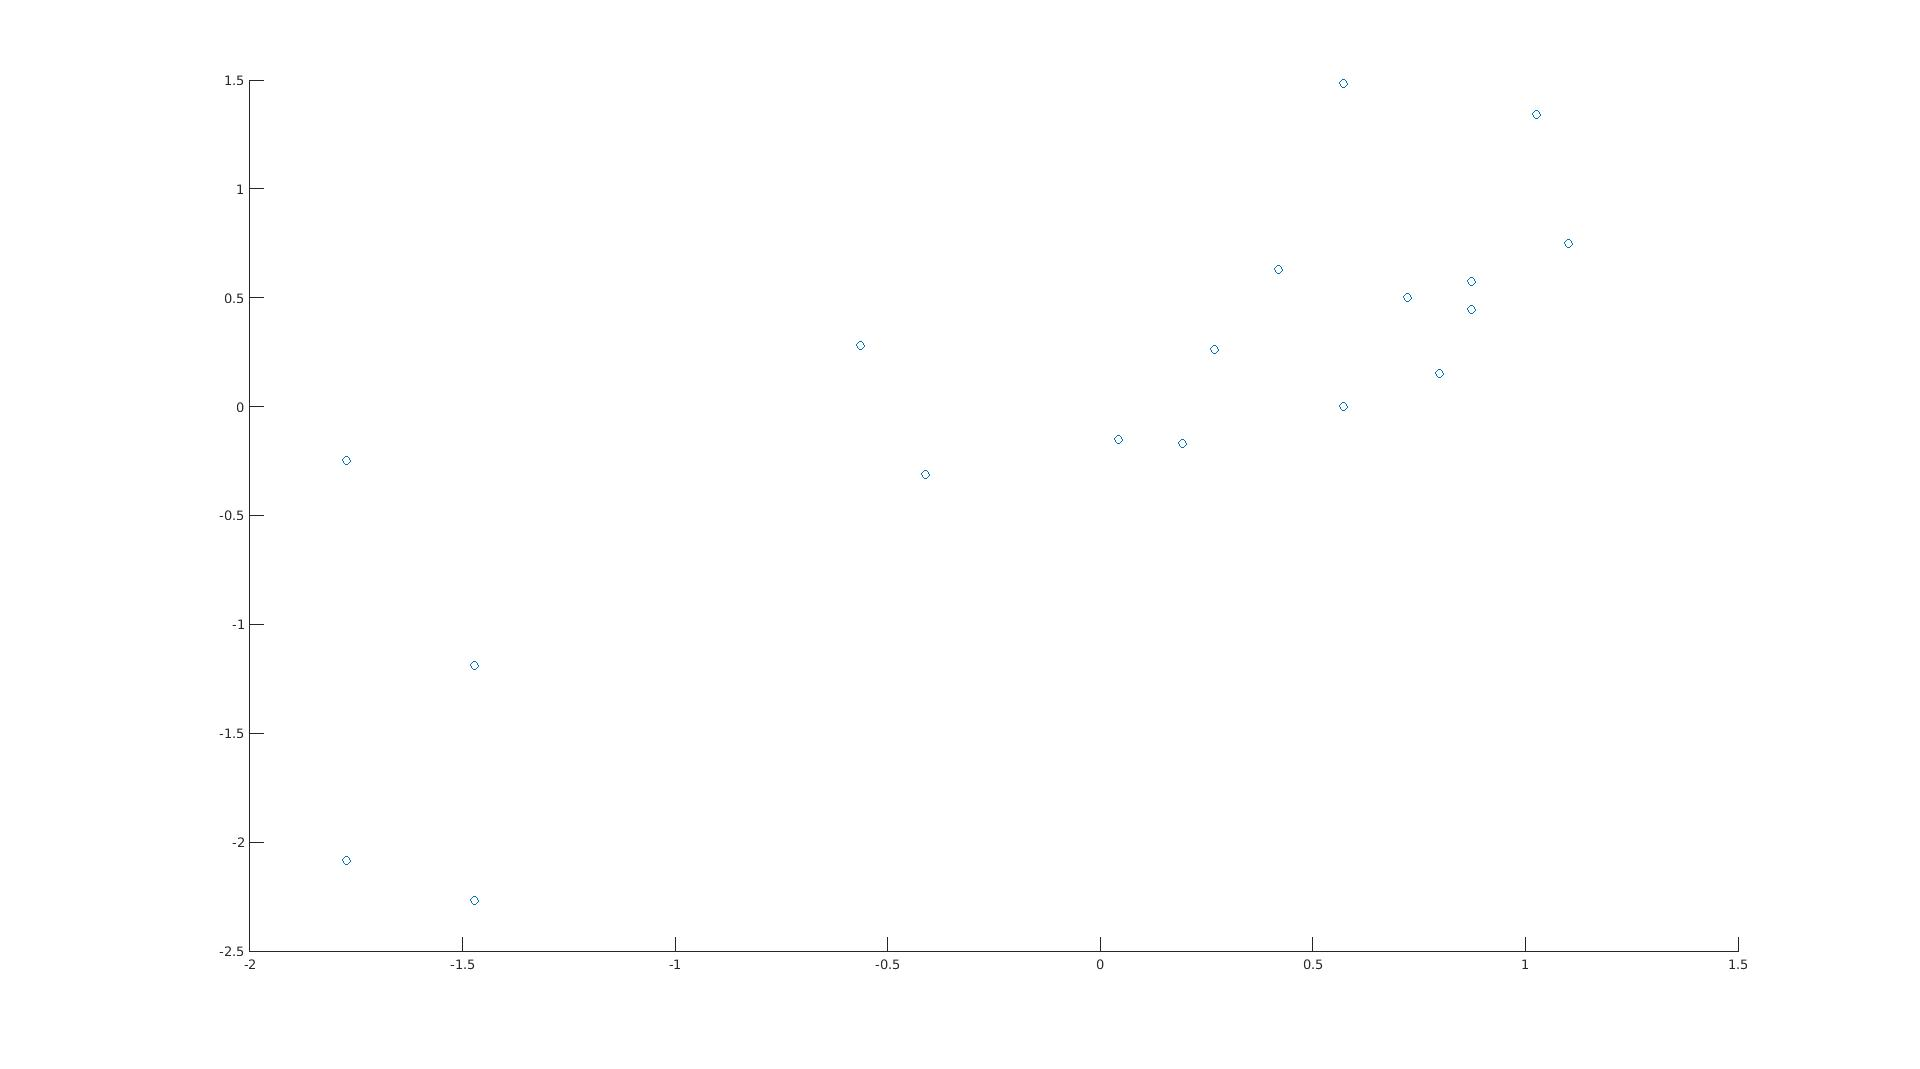
\includegraphics[scale=0.26]{task3_2.jpg}
	\caption{Fitness-Plot}
\end{figure}

\section*{4}
\begin{enumerate}
	\item als Pre-Processing Algorithmus wird die Principal Component Analysis (PCA) benutzt
	\item Es gibt 36 000 $ \cdot $ 19 Eigenfaces. Ein Bild hat 360000 Bildvektoren (bei einer Auflösung 200x180) und es werden 19 Bilder benutzt ( 20 - "original\")
	\item Der Durchschnitt der Eigenfaces sieht wie ein Übereinanderlegen von mehren  Bildern aus. Es keine klare Person zu erknnen. Bei den Eigenfaces erkennt man bei den treffen eigenfaces (zu der Person) klare Konturen besonders im Bereich der Nase und der Augen sowie der Kopfform. Nicht passende Bilder wirken stark verwaschen und undeutlich.
Die Rekonstrukiton von Person im Training ist deutlich besser als die ohne. Besonders auffallend ist eine gute Rekonstruktion der Kopfform, der Ohren sowie der Nase und des Kinnes.
\end{enumerate}

\end{document}

